
% This LaTeX was auto-generated from MATLAB code.
% To make changes, update the MATLAB code and republish this document.

\documentclass{article}
\usepackage{graphicx}
\usepackage{color}

\sloppy
\definecolor{lightgray}{gray}{0.5}
\setlength{\parindent}{0pt}

\begin{document}

    
    
        \color{lightgray} \begin{verbatim}Mat File: AAPlantD1_2GHz_TX1_hpol_run4
Frequency: 2.245000e+00
Location: AA Plant Day 1 at Automotive Assembly Plant
RX Antenna: Omni-directional, Cross Pol
RX Antenna Gain: -4.200000e+00
TX Antenna: Omni-directional, V Pol
TX Antenna Gain: 2.900000e+00
TX Power, Watts: 1.500000e+00
PN Oversample Factor: 
Sample rate, MHz: P
Frequency: 2.245000e+00
\end{verbatim} \color{black}
    
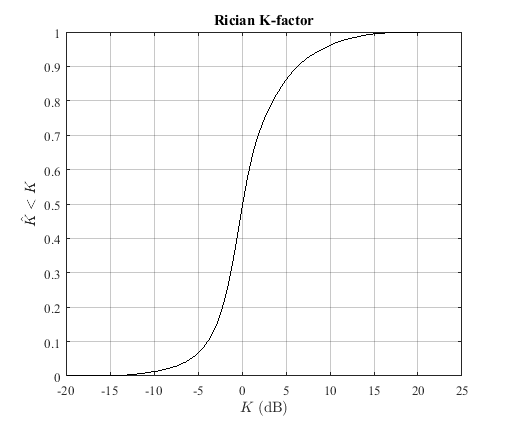
\includegraphics [width=4in]{make_report_01.eps}

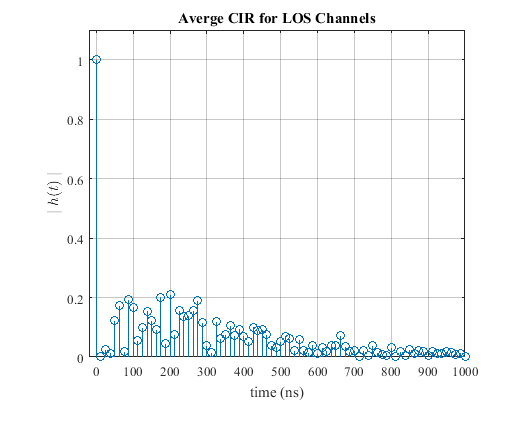
\includegraphics [width=4in]{make_report_02.eps}

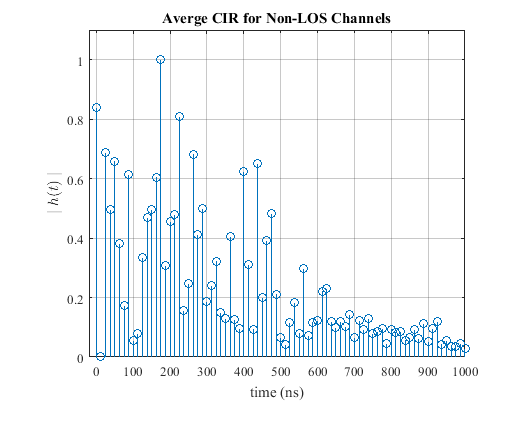
\includegraphics [width=4in]{make_report_03.eps}

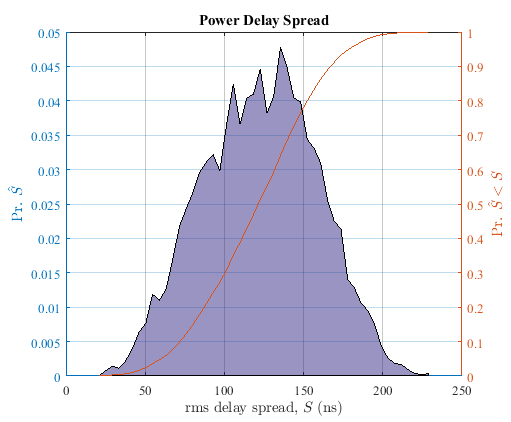
\includegraphics [width=4in]{make_report_04.eps}

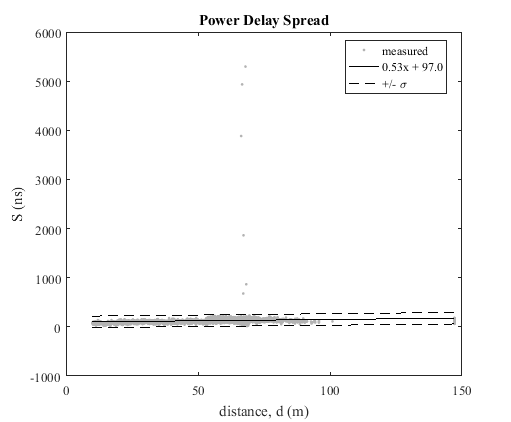
\includegraphics [width=4in]{make_report_05.eps}

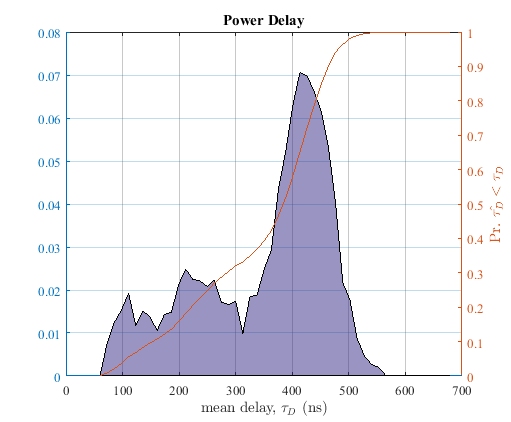
\includegraphics [width=4in]{make_report_06.eps}

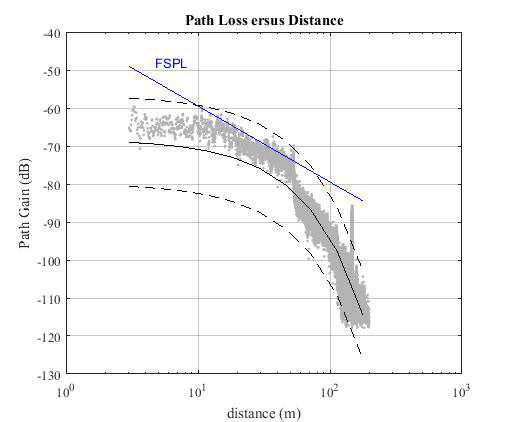
\includegraphics [width=4in]{make_report_07.eps}



\end{document}
    
